\chapter{Introduction} \label{ch:Introduction}

% Please add the following required packages to your document preamble:
% \usepackage{longtable}
% Note: It may be necessary to compile the document several times to get a multi-page table to line up properly
\begin{longtable}{|l|r|}
\caption{Wind turbine geometrical specifications}
\label{tab:turbinegeometry}\\
\hline
\multicolumn{1}{|c|}{\textbf{Variable}} & \multicolumn{1}{c|}{\textbf{Value}} \\ \hline
\endhead
%
Radius (R)                              & 50 {[}m{]}                          \\ \hline
Number of Blades                        & 3                                   \\ \hline
Blade starts at                         & 0.2 r/R                             \\ \hline
Twist                                   & 14*(1-r/R) {[}degrees{]}            \\ \hline
Blade Pitch                             & -2 {[}degrees{]}                    \\ \hline
Chord Distribution                      & 3*(1-r/R)+1 {[}m{]}                 \\ \hline
Airfoil                                 & DU 95-W-180                         \\ \hline
Rotor yaw angle                         & 0, 15 and 30 {[}degrees{]}          \\ \hline
\end{longtable}

% Please add the following required packages to your document preamble:
% \usepackage{longtable}
% Note: It may be necessary to compile the document several times to get a multi-page table to line up properly
\begin{longtable}{|l|l|}
\caption{Wind turbine operational specifications}
\label{tab:operspecs}\\
\hline
\textbf{Variable}        & \textbf{Value}          \\ \hline
\endhead
%
Wind speed (U0)          & 10 {[}m/s{]}            \\ \hline
Tip speed ratio ($\lambda$) & 6, 8, 10                \\ \hline
Rotor yaw angle          & 0, 15, 30 {[}degrees{]} \\ \hline
\end{longtable}

\begin{figure}
    \centering
    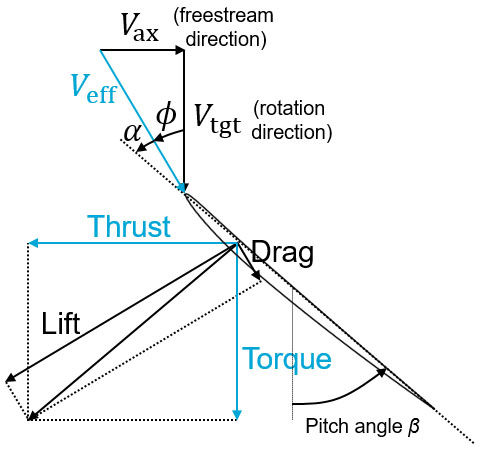
\includegraphics[width=0.5\textwidth]{Figures/velocitydiagram.jpg}
    \caption{Caption}
    \label{fig:enter-label}
\end{figure}